\documentclass[aspectratio=169]{beamer}
\usetheme{Madrid}
\usepackage[utf8]{inputenc}
\usepackage[T1]{fontenc}
\usepackage{tikz}
\usepackage{amssymb}
\usepackage{graphicx}
\setbeamertemplate{navigation symbols}{}
\setbeamercolor{title}{fg=white,bg=magenta!70!red}
\setbeamercolor{frametitle}{fg=white,bg=magenta!70!red}
\setbeamercolor{block title}{bg=magenta!70!red!20,fg=black}
\setbeamercolor{block body}{bg=magenta!70!red!8,fg=black}
\setbeamercolor{item}{fg=magenta!70!red}
\setbeamercolor{itemize item}{fg=magenta!70!red}
\setbeamertemplate{itemize item}[triangle]

\title{Foundations 5 — Images}
\subtitle{Pixels, resolution, bit depth --- a picture is just more binary}
\author{ByteForge --- Grade 9 --- The Deep Diver}
\date{}

\begin{document}

\begin{frame}
    \titlepage
\end{frame}

\begin{frame}{Today's Missions}
    \Large
    \begin{itemize}
        \item Learn: What Is a Digital Image?
        \item Count the Lit Pixels
        \item Which Row Has the Most Light
    \end{itemize}
\end{frame}

\begin{frame}{An image is really just a grid of numbers}
    \large
    \begin{itemize}
        \item Zoom into any real photo far enough and you see individual squares --- pixels
        \item A computer "draws" the image by reading that grid and colouring each pixel
        \item There is no picture "drawn" anywhere --- it is genuinely just numbers
    \end{itemize}
\end{frame}


\begin{frame}{Monochrome --- the simplest case, 1 bit per pixel}
    \large
    \begin{itemize}
        \item Black-and-white needs only ONE bit per pixel: 0 = dark, 1 = lit
        \item "0110" is four pixels in a row: dark, lit, lit, dark
    \end{itemize}
\end{frame}


\begin{frame}{More bits per pixel = more possible colours}
    \large
    \begin{itemize}
        \item 1 bit = only 2 possibilities (0 or 1)
        \item 8 bits = 256 shades of grey
        \item 24 bits (8 each for red/green/blue) = over 16 million real colours
        \item More bits = more detail, but also a bigger file
    \end{itemize}
\end{frame}

\begin{frame}{Real-World Examples}
    \large
    \begin{itemize}
        \item Every photo on your phone is millions of pixels, each one just 3 numbers (red, green, blue) --- exactly this chapter's idea, at real-world scale.
        \item An old black-and-white video game (1 bit per pixel) genuinely takes up far less storage than a modern photo (24+ bits per pixel) --- same grid idea, wildly different bit depth.
    \end{itemize}
\end{frame}


\begin{frame}{Image}
    \begin{center}
    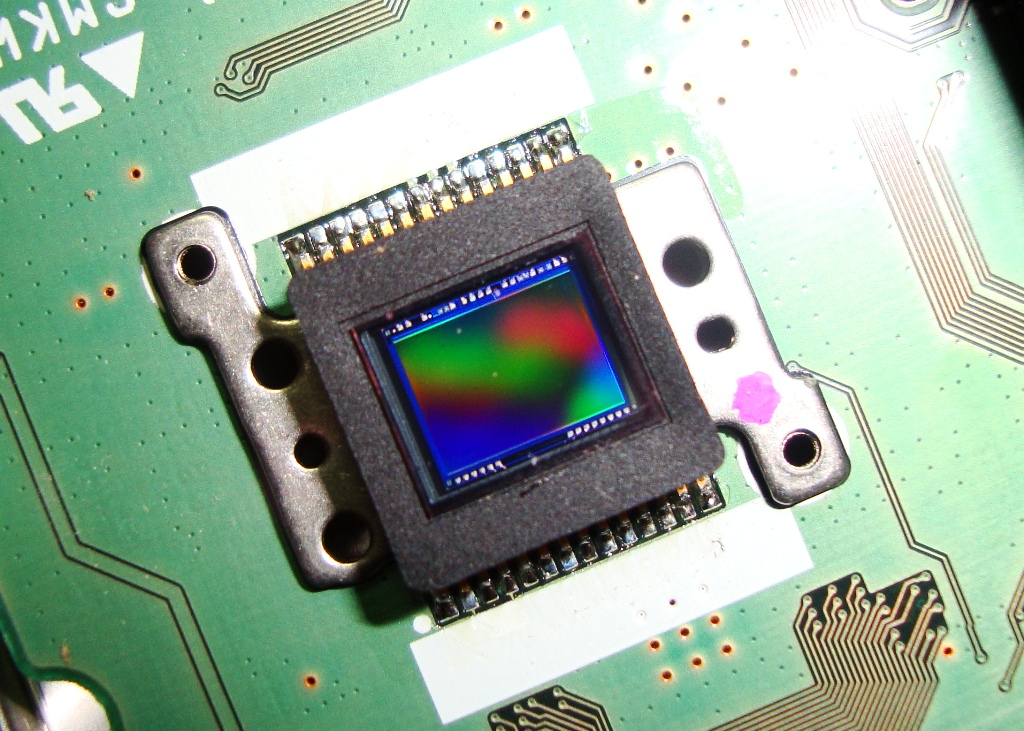
\includegraphics[width=0.5\textwidth]{images/sensor.jpg}

    \large A real camera sensor --- each of those tiny squares captures ONE pixel's worth of colour.

    \small CCD image sensor --- Ahmed2IQ, public domain, via Wikimedia Commons
    \end{center}
\end{frame}

\begin{frame}{Let Them Discover}
    \large
    Zoom WAY into any photo on a phone or computer until you can see individual squares. Count how many different colours you can spot in just a small patch --- that is bit depth, visible.
\end{frame}

\begin{frame}{Your Turn}
    \Large
    Open the mission map, find \textbf{Foundations 5 — Images}, and fly it for real ---
    everything you just saw, you now do yourself.
\end{frame}

\end{document}
